%!TEX root =  main.tex
\chapter[Scaling partitioned replicated systems]{Scaling partitioned replicated systems}

Replication refers to the technique of managing redundant data on a set of
servers (replicas) in a way to ensure that each replica of the service keeps a
consistent state, given a consistency criterion. Over more than three
decades, replication has been an area of interest and has been studied in
many domains, such as database systems, file systems, and 
distributed object systems. Although replication is often used to achieve high
availability, replication can also help improve performance.
Availability is the capability of a system to continue to work, even in the
presence of failures, as long as the number of failures is below a given
threshold. Performance refers to the throughput and response time of the 
system. For instance, a service that serves mainly read operations can distribute the
requests to the different replicas. Each replica can then process requests in
parallel and improve the throughput and the response of the system. 

Conceptually, replication can be categorized into two main categories: full and
partial replication. Full replication means that the whole state of the service
is available on all replicas, while in partial replication, each replica only
contains a subset of the state. For example, in a distributed database, full
replication means that all rows of a table are available on all replicated servers,
while partial replication means that some replicas contain only a subset of the rows.
Intuitively, full replication often comes at a higher cost. If all replicas have
to keep the whole same state and execute the same sequence of commands, the system
cannot scale under update operations. It may also become infeasible to have a full copy of the system's
state when data continually grows, as the replicas may not have enough space to store
it (i.e., typically in main memory databases). Therefore, increasing the number of replicas in a fully replicated system
results in bounded improvements in performance. The main idea
of partial replication is that not all replicas have to process each request. The
replicas in a partially replicated system only store a subset of the state and
handle requests that involve that data, thus providing the potential for scalable performance.
However, the main challenge is how to keep the replicas in a partially replicated system
consistent. In this chapter, we will survey several approaches to replication
and scaling the performance of a replicated system.

\section{Full replication schemes}

Replication has become a standard approach to fault tolerance: if one server
fails, another one takes over. In a fully replicated system, every server
replicates a full copy of the service's state. All replicas use an algorithm
that ensures data coherence across all these nodes. Although there are many
replication techniques \cite{Replication:book}, there are two major classes
of replication techniques that have become widely known to ensure strong
consistency: \emph{active replication} and \emph{passive replication}.


\subsubsection{Active replication} 
With the \emph{active replication} (also called state machine replication) approach,
client requests are sent to all members of a given group of replicas
in the same order. The replicas will then execute the requests as though they
were the only member of the group, to reach the same state, and reply to the
client. If a client sends a request to a group of $n$ replicas (assuming no
failures), then the client will receive $n$ identical replies to the 
request. With this replication scheme, a crash does not increase the latency
experienced by the client. State machine replication is a fundamentally powerful
building block that enables the implementation of highly available distributed
services by replication. 
%State machine replication achieves strong consistency
%(i.e., linearizability) by regulating how client commands are propagated to and
%executed by the replicas: every non-faulty replica must receive and execute
%every command deterministically and in the same order. 
Some other replication schemes, such as chain replication \cite {chainreplication,
chainreplication:byzantine}, multi-primary replication, and deferred-update replication
\cite{sciascia2012sdur, Replication:book, chundi96dur} are based on state machine replication.

\subsubsection{Passive replication} 
In the \emph{passive replication} (also called \emph{primary-backup}) approach,
the requests are sent to only one member of the replica group (the
\emph{primary}), while all other members are \emph{backups}. The primary will execute
each request and send the response to the client. Any modifications to the
primary's state is updated to other members of the group (the backups). If the
primary fails, one of the backups takes over the service by becoming a new
primary. Unlike the active replication approach, passive replication does not
waste resource on redundant execution of requests, and allows non-deterministic
requests. However, a failure on the leader will affect the latency of a command.

In~\cite{pedone:replication}, the authors presented a
framework to compare and distinguish replication protocols in databases
and distributed systems (Figure~\ref{fig:replication:org}). This model
classifies replication protocols by five generic steps of replication as
following:

\begin{figure*}[ht!]
  \begin{minipage}[b]{1.0\linewidth}
  \centering
        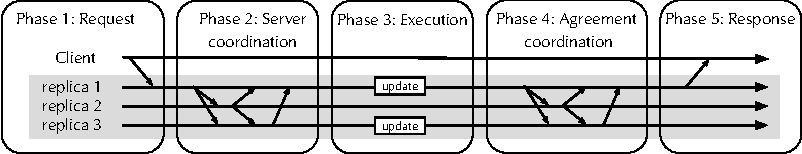
\includegraphics[width=1\linewidth]{figures/replication-original}
  \end{minipage}
  \caption{Functional model with the five phases}
  \label{fig:replication:org}
\end{figure*}

\begin{itemize}
  \item \textit{Request phase (RE):} In the request phase, a client submits an
     operation to the system by sending the request to one ore more replicas.
  \item \textit{Server coordination phase (SC):} The replicas coordinate
  with each other to synchronize the execution of the request.
  \item \textit{Execution phase (EX):} The operation is executed on the replica servers.
  \item \textit{Agreement coordination phase (AC):} The replica servers
  coordinate to agree on the result of the execution.
  \item \textit{Response phase (END):} The result of the operation is
  transmitted back to the client.
\end{itemize}

The differences between different replicated systems come from the different
ways in which each phase is implemented. In some cases, a phase could be omitted (e.g.,
when messages are ordered by an atomic multicast/broadcast primitive in the
ordering phase (\emph{SC}), it is not necessary to run the agreement
coordination (\emph{AC}) phase). With this generic functional model, the
involved steps in the active replication technique can be depicted as follows
(Figure \ref{fig:replication:active}):

\begin{figure*}[ht!]
  \begin{minipage}[b]{1.0\linewidth}
  \centering
        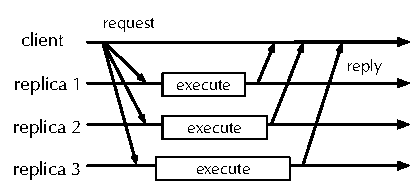
\includegraphics[width=1\linewidth]{figures/replication-active}
  \end{minipage}
  \caption{Communication steps involved in active replication}
  \label{fig:replication:active}
\end{figure*}

\begin{enumerate}
  \item The client submits the request to the server by using an atomic
  broadcast primitive.
  \item Server coordination is given by the total order property of the Atomic
  Broadcast.
  \item All replicas deterministically execute the request in the order they are
  delivered.
  \item There is no coordination required after the execution. All replicas
  should reach the same state.
  \item All replicas send the reply to the client.
\end{enumerate}

The involved steps in the passive replication technique can be depicted
according to the generic functional model as follows (Figure
\ref{fig:replication:passive}):

\begin{figure*}[ht!]
  \begin{minipage}[b]{1.0\linewidth}
  \centering
        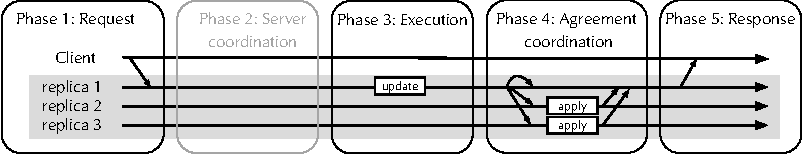
\includegraphics[width=1\linewidth]{figures/replication-passive}
  \end{minipage}
  \caption{Communication steps involved in passive replication}
  \label{fig:replication:passive}
\end{figure*}

\begin{enumerate}
  \item The client submits the request to the primary.
  \item Server coordination is not required.
  \item The primary is the only process that executes the request.
  \item The primary coordinates with the backups by broadcasting the update
  information.
  \item The primary sends the reply to the client.
\end{enumerate}


% \begin{figure*}[ht!]
%   \centering
%   \begin{subfigure}[b]{0.49\textwidth}
%     \centering
%     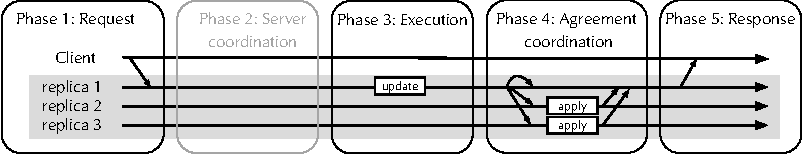
\includegraphics[width=1\columnwidth]{figures/replication-passive}
%     \caption{Passive replication}
%     \label{fig:replication:passive}
%   \end{subfigure}
%   \begin{subfigure}[b]{0.49\textwidth}
%     \centering
%     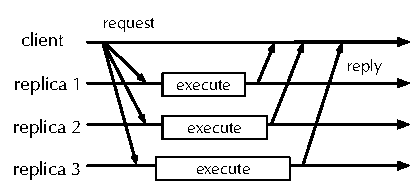
\includegraphics[width=1\columnwidth]{figures/replication-active}
%     \caption{Active replication}
%     \label{fig:replication:active}
%   \end{subfigure}
%   \caption{Replication techniques}
%   \label{fig:replication}
% \end{figure*}

\section{Partial replication schemes}

Full replication ensures the update of every operation to be replicated on
every replica in the system. This prevents the system from scaling with the
increase in the number of replicas. In fact, the performance of the system is
limited by the performance of a single replica. Partial replication addresses
these issues by replicating only a subset of data at each replica. Therefore,
different subsets of data can be accessed and updated concurrently. 
% In other words, scalable performance can be achieved with state partitioning.

Partitioning is a technique that divides the state of a service in multiple
partitions so that most commands access one partition only and are equally
distributed among partitions. Partitioned replicated systems can provide highly
scalable and available systems; however, they introduce other challenges. Most
services cannot be ``perfectly partitioned''; that is, the service state cannot
be divided in a way that commands access one partition only. Therefore, a
partitioning protocol must cope with multi-partition commands. In database
systems, partitioning is usually referred to as \emph{sharding}, where the dataset
is divided into horizontal fragmentation, known as partitions. Each partition
essentially has the same schema and columns but contains different subsets of
the total data set. The partitions are then distributed across separate database
servers, referred to as physical shards, which can hold multiple logical
partitions. Those physical shards can be replicated to tolerate failures. 
Despite this, the data held within all the partitions collectively
represent an entire logical dataset. 

To guarantee consistency across multiple replicas of the data, a consensus
protocol (e.g., Paxos~\cite{reference_here}, Raft~\cite{reference_here}) is used. 
Essentially, this protocol works as a quorum
mechanism. Any change to the dataset requires a majority of replicas to agree to
the change. Google Spanner~\cite{corbett2013spanner} and Calvin \cite{calvin}
are two database solutions in this category. Both systems were designed
to be highly scalable distributed relational databases. The main difference
between the two systems is that Spanner uses two-phase commit as an agreement
protocol to synchronize the changes between partition, without the need of
server coordination before the execution, while Calvin uses a single, global
consensus protocol per database to synchronize transactions before the execution.
All involved replicas of Calvin then deterministically execute and commit the
transaction, without an agreement protocol. The next sections will describe how
those database systems work. In addition, we will detail Scalable State
Machine Replication, a system in the third category, which requires both server
coordination and agreement for providing a strong consistency guarantee.



% Partitioning
% replicated state machine can provide highly scalable and available systems;
% however, introduce other challenges. Most services cannot be ``perfectly
% partitioned''; that is, the service state cannot be divided in a way that
% commands access one partition only. Therefore, a partitioning protocol must cope
% with multi-partition commands.


In general, we can model partitioned replication protocols by
extending the five-phase functional model in \cite{pedone:replication} to
include the coordination between components in a partitioned replicated system
(see Figure \ref{fig:replication:coordination}). Those phases are:


\begin{figure*}[ht!]
  \begin{minipage}[b]{1.0\linewidth}
  \centering
        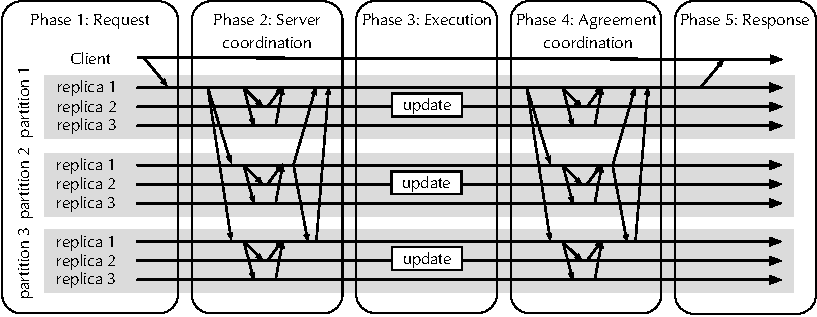
\includegraphics[width=1\linewidth]{figures/replication-coordination}
  \end{minipage}
  \caption{Coordination in a partitioned replicated system}
  \label{fig:replication:coordination}
\end{figure*}

\begin{itemize}
  \item \textit{Request phase (RE):} In the request phase, a client submits the request
     to the system. This can be done in different ways: the request could
  be sent to all servers involved in the request or to one server/partition, which would
  then forward the request to the other processes. In any case, the client should
  be able to identify the involved partitions that contain the data accessed by
  the request. The client can send the request directly or use a proxy layer to
  handle the transmission.
  \item \textit{Server coordination phase (SC):} The replicas of all partitions
  that contain the data required by the request will coordinate with each other
  to synchronize the execution of the request. Depending on the consistency level,  
  concurrent requests will be ordered within and/or across the involved partitions.
  \item \textit{Execution phase (EX):} The involved servers execute the request.
  \item \textit{Agreement coordination phase (AC):} The servers of all involved
  partitions agree on the outcome of the execution.
  \item \textit{Response phase (END):} The result of the request is sent back to the client.
\end{itemize}

\subsection{Agreement coordination without server coordination}

Spanner is a NewSQL \cite{Grolinger:2013tp} globally distributed database system
developed by Google \cite{corbett2013spanner}. Spanner provides features such as
global transactions, strongly consistent reads, and automatic multi-site
replication and automatic failover. Spanner partitions data into multiple shards, and
replicates every shard via Paxos across independent regions for high
availability. So, every operation in a transaction is a replicated operation
within a Paxos replicated state machine.

Spanner consists of multiple \emph{zones}, each of which is a deployment of
Bigtable servers. A zone uses one \emph{zonemaster} to assign data to one
hundred to several thousand sets of partitions. Each partition is a set of
Paxos-based state machines (so-called \emph{spanservers}).  To implement
transactions, including transactions that span across multiple partitions, Spanner
uses two-phase locking, for concurrency control, and two-phase commit, for transaction termination. Each
spanserver implements a lock table to support two-phase-locking and a
transaction manager to support distributed transactions. Operations that
require synchronization have to acquire a lock from the lock table. The Paxos
leader in each partition is responsible for participating in these protocols on
behalf of that partition. Clients in Spanner use per-zone \emph{location
proxies} to locate the spanservers assigned to serve their data. To order the
transaction between partitions, Spanner uses TrueTime API, a combination of GPS
and atomic clocks in all of their regions (i.e., zones) to synchronize time 
within a known uncertainty bound. If two transactions are processed during time
periods that do not have overlapping uncertainty bounds, Spanner can be certain
that the later transaction will see all the writes of the earlier transaction.

\begin{figure*}[ht!]
  \begin{minipage}[b]{1.0\linewidth}
  \centering
        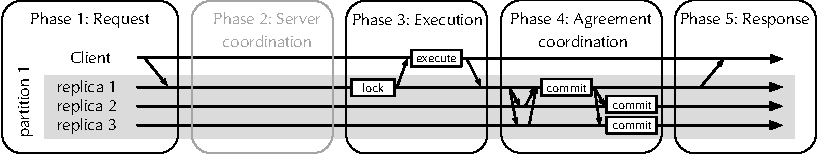
\includegraphics[width=1\linewidth]{figures/spanner-single-partition}
  \end{minipage}
  \caption{Coordination in single-partition transactions in Spanner}
  \label{fig:spanner-single-partition}
\end{figure*}

\subsubsection{Single-partition transactions}
 
In Spanner, if a transaction accesses data in a single partition (single-shard
transaction), Spanner processes that transaction as follows (see
Figure~\ref{fig:spanner-single-partition}). First, the client process queries
the location proxy to determine which partitions store the data accessed by the
transaction and send the transaction to the Paxos leader of that partition. The
leader acquires the read locks on the involved objects and acknowledges the
client. The client executes the transaction, then initiates the commit on the
leader. The leader then coordinates with other replicas in its Paxos group to
commit the transaction, and responds to the client.

\begin{figure*}[ht!]
  \begin{minipage}[b]{1.0\linewidth}
  \centering
        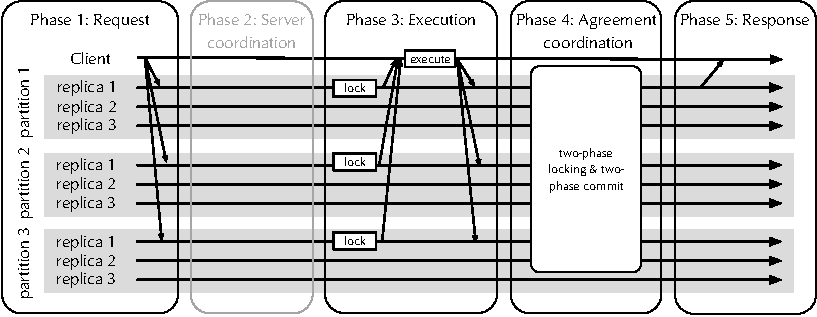
\includegraphics[width=1\linewidth]{figures/spanner-multi-partition}
  \end{minipage}
  \caption{Coordination of multi-partition transactions in Spanner}
  \label{fig:spanner-multi-partition}
\end{figure*}

\subsubsection{Multi-partition transactions} 
In the case the transaction accesses more than a single partition, the leaders
of all involved partitions have to coordinate and perform a two-phase commit to
ensure consistency and use two-phase locking to ensure isolation (see
Figure~\ref{fig:spanner-multi-partition}). First, the client needs to
determine the involved partitions by querying a location proxy. Then, the client
sends the transaction to the leader of each involved group, which acquires read
locks and returns the most recent data. The client then performs the execution
of the transaction locally. To commit the transaction, the client chooses a
coordinator from the set of involved leaders, then initiates the commit by sending a
commit message to each leader, together with the information of the coordinator.
On receiving the commit message from the client, the involved leaders coordinate to
acquire write locks by performing two-phase locking followed by two-phase
commit. After having the transaction committed on all involved partitions, the
coordinator leader sends a response to the client.

In general, the transaction processing of Spanner can be mapped to the
coordination protocol in Figure~\ref{fig:replication:coordination} as follows:
\begin{enumerate}
  \item Client sends the transaction to the Paxos leader process.
  \item There is no initial coordination required between involved replicas.
  \item The leader(s) acquires locks and retrieves data for the client. The client
  executes the transaction and initiates the commit protocol.
  \item The leader(s) coordinates with other leaders to commit the transaction.
  \item The leader sends the response to the client.
\end{enumerate}

Spanner allows data to be re-sharded across
\emph{spanservers}, or \emph{zones} data centers, to balance loads and in response
to failures by the \emph{placement driver}~\cite{reference_here}. Periodically, the \emph{placement driver}
communicates with spanservers to re-arrange data. During these transfers,
clients can still execute transactions (including updates) on the database.

\subsection{Server coordination without agreement coordination}

Calvin is a distributed transaction protocol that consists of a transaction
scheduling and replication management layer for distributed storage systems
\cite{calvin}. Similar to Spanner, Calvin also shards its data on multiple
partitions for performance, and replicates those partitions for availability. The
main difference between the two systems is the way Calvin deals with the problem
of transaction synchronization. Spanner solves the problem in a traditional
way (i.e., two-phase locking and two-phase commit) and reduces the cost of synchronization
by decreasing the time during which transactions hold locks using
TrueTime API.

By executing transactions using two-phase locking and two-phase commit, 
traditional database systems have no a priori deterministic transaction order. 
This means that the servers do not need to ensure some transaction order defined before the execution of the
transaction. Calvin chooses to use a deterministic transaction order. This
approach could remove the overhead of coordinating after the execution phase,
since all the nodes execute the same sequence of input transactions in a deterministic way,
to produce the same output. Calvin achieves deterministic order by using
a sequencer (\emph{preprocessing}) to let replicas agree on the execution order and
transaction boundaries.

Client processes in Calvin first submit transactions to a distributed,
replicated log before the transactions are sent to partitions for execution. The sequencer then
processes this request log, determines the order in which transactions are
executed, and establishes a global transaction input sequence. Then, each replica
simply reads and processes transactions from this global order (Figure
\ref{fig:calvin}).

\begin{figure*}
  \begin{minipage}[b]{1.0\linewidth}
  \centering
        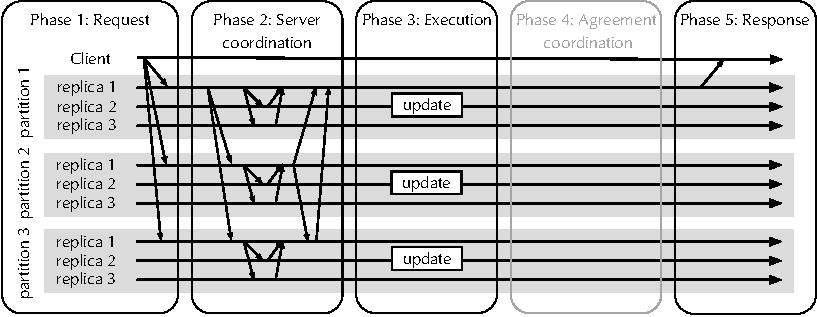
\includegraphics[width=1\linewidth]{figures/calvin}
  \end{minipage}
  \caption{Transaction processing in Calvin}
  \label{fig:calvin}
\end{figure*}

Essentially, Calvin can be described in the following steps, according to
the framework of coordination protocol in
Figure~\ref{fig:replication:coordination}:

\begin{enumerate}
  \item Client submits the transaction to the sequencer nodes.
  \item Sequencers coordinate to order and schedule the execution of the transaction in a global sequence.,
  \item The involved replicas execute the same sequence of transactions, produce the same output.
  \item As all the replicas reach the same state, no agreement coordination is necessary.
  \item The replicas send the response to the client.
\end{enumerate}

\subsection{Server coordination with agreement coordination}
\label{sec:ssmr}
Scalable State Machine Replication (\ssmr) is an extension to state machine replication (SMR) that under
certain workloads allows performance to grow proportionally to the number of
replicas. \ssmr\ partitions the service state and replicates each partition. It
relies on an atomic multicast primitive to consistently order commands within
and across partitions. In addition, \ssmr\ assumes a static workload
partitioning. Any state reorganization requires system shutdown and manual
intervention.

In S-SMR~\cite{bezerra2014ssmr}, the service state \vvt\ is composed of $k$
partitions, in set $\Psi = \{\mathcal{V}_1, ..., \mathcal{V}_k\}$. Server group
$\ssm_i$ is assigned to partition $\mathcal{V}_i$. For brevity, we say that
server $s$ belongs to $\mathcal{V}_i$ meaning that $s \in \ssm_i$, and say
``multicast to $\mathcal{V}_i$'' meaning ``multicast to server group $\ssm_i$''.
S-SMR relies on an \emph{oracle}, which tells which partitions are accessed by
each command.\footnote{The oracle returns a set with the partitions accessed
by the command, but this set does not need to be minimal; it may contain all
partitions in the worst case, when the partitions accessed by the command cannot
be determined before the command is executed.}

\begin{figure*}
  \begin{minipage}[b]{1.0\linewidth}
  \centering
        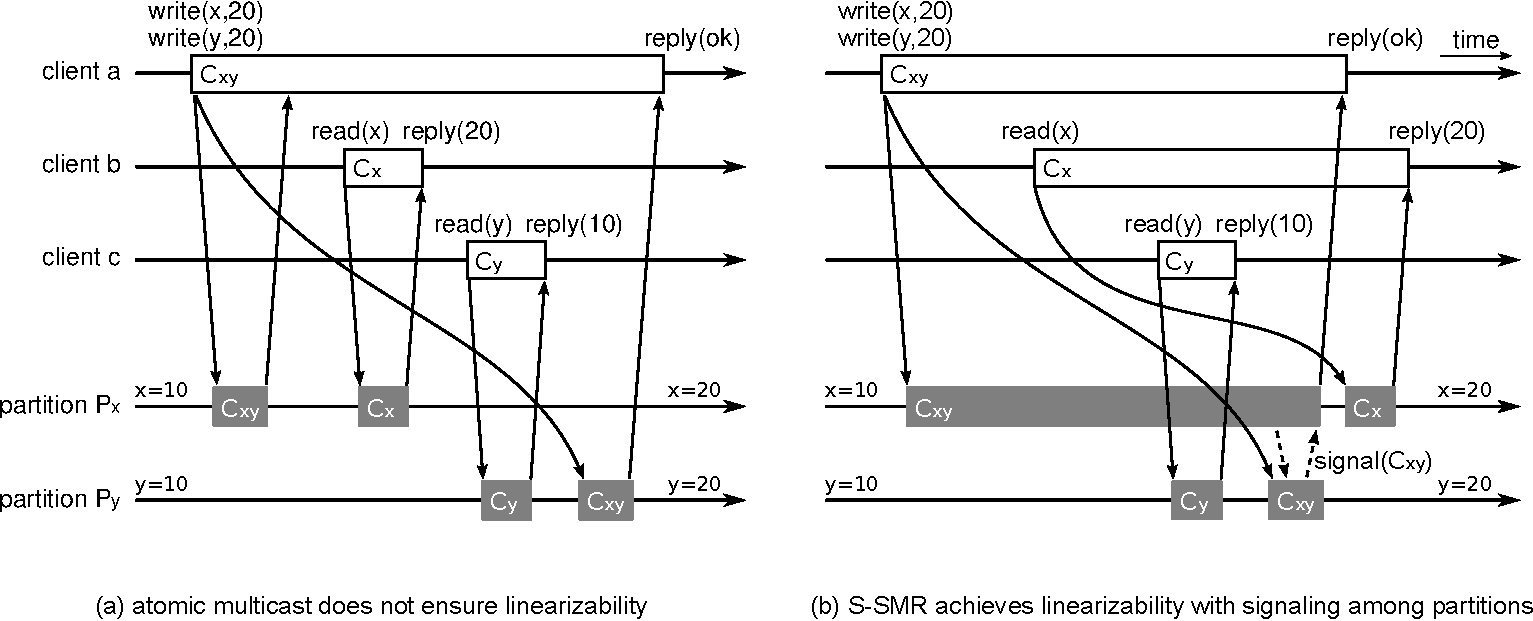
\includegraphics[width=1\linewidth]{figures/ssmr}
  \end{minipage}
  \caption{Atomic multicast and S-SMR (for simplicity, there is a single replica per partition)}
  \label{fig:ssmr}
\end{figure*}

To execute a command, the client multicasts the command to the appropriate
partitions, as determined by the oracle. Commands that access a single partition
are executed as in classical SMR: replicas of the concerned partition agree on
the execution order and each replica executes the command independently. In the
case of a multi-partition command, replicas of the involved partitions deliver
the command and then may need to exchange state in order to execute the command
since some partitions may not have all the values read in the command. This
mechanism allows commands to execute seamlessly despite the partitioned state.

S-SMR improves on classical SMR by allowing replicated systems to scale, while
ensuring linearizability. Under workloads with multi-partition commands,
however, it has limited performance, in terms of latency and throughput
scalability. Such decreased performance when executing multi-partition commands
is due to partitions (i) exchanging state variables and (ii) synchronizing by
exchanging signals. Thus, the performance of \ssmr\ is particularly
sensitive to the way the service state is partitioned.

One way to reduce the number of multi-partition commands is by dynamically
changing the partitioning, placing variables that are usually accessed together
in the same partition. However, the partitioning oracle of \ssmr\ relies on a
static mapping of variables to partitions. One advantage of this implementation
is that all clients and servers can have their own local oracle, which always
returns a correct set of partitions for every query. Such a static mapping has
the major limitation of not allowing the service to dynamically adapt to
different access patterns.

In summary, the following steps are involved in the processing of a request in
\ssmr\, according to our functional model.

\begin{enumerate}
  \item Client sends the requests to the servers of all involved partitions.
  \item Server coordination is given by the total order property of the Atomic
  multicast.
  \item All involved replicas execute the requests in the order they are delivered.
  \item Partitions exchanges signals to ensure linearizability.
  \item All replicas send back the result to the client, and the client
  typically only waits for the first answer.
\end{enumerate}

\begin{figure*}
  \begin{minipage}[b]{1.0\linewidth}
  \centering
        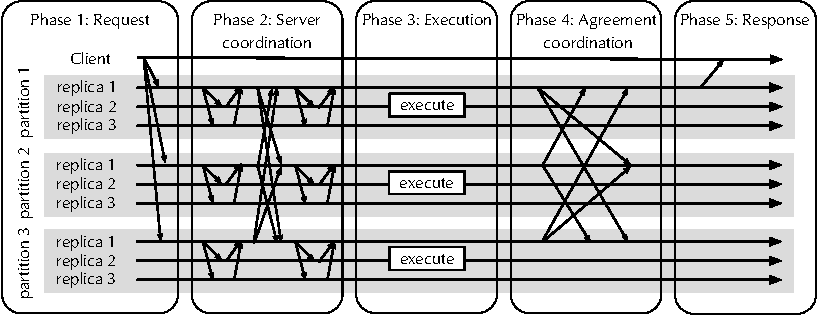
\includegraphics[width=1\linewidth]{figures/coordination-ssmr}
  \end{minipage}
  \caption{Atomic multicast and S-SMR (for simplicity, there is a single replica per partition)}
  \label{fig:coordination-ssmr}
\end{figure*}

\section{Conclusion}

In this chapter, we surveyed a number of approaches to replication and
partitioning of a replicated system. Replication and partitioning are widely used
by several system, from databases, file systems to distributed object systems.
We introduced an abstract framework that identifies five basic coordination
steps in a partitioned replicated system. This framework allows us to give an
insight of design choices of several approaches in the literature. By
understanding these approaches, we came up with techniques that aim to
minimize the overhead of cross partition coordination, thus providing better
performance scalability.
We discuss these techniques in the next chapters.













% \section{Replication and partitioning}
% \section{Scaling in distributed database systems}


% \subsection{Google Spanner}

% \subsection{Calvin}

% \section{Execution models}

% In Spanner, clients can build applications by issuing multiple read and
% write requests to servers and encapsulating multiple requests into a
% transaction, which can also contain client-side arbitrary computation on the
% data. When the client commits the transaction, if the transaction spans across
% multiple partitions, one of the involved partitions plays the role of the
% coordinator to perform two-phase commit with the other groups for committing the
% transaction. Thus, transactions in Spanner’s execute-coordinate model may abort.

% In state machine replication, the application logic runs entirely at the
% replicas; clients simply invoke the operations (similar to database stored
% procedures). State machine replication relies on an atomic multicast protocol to
% totally order client requests within and across involved partitions. Each
% replica simply reads and processes requests as in the order it delivers them.
% This model makes sure the executions of requests will never abort.


% \section{Scaling state machine replication with S-SMR}

% Broadly speaking, there are two classes of techniques for scaling state machine
% replication by partitioning: \emph{static} and \emph{dynamic}.
% Figure~\ref{fig:motivation} shows the result of a motivating experiment that
% compares two representative systems, one of each class. In the experiment, we
% measured the throughput and number of state moves over time with two different
% workloads: one with strong locality and one with weak locality. The workloads
% are inspired by the social network Twitter, in which the network is modeled as a
% graph, and users can ``post'' messages. The social graph was generated using a
% Zipfian distribution, where the Zipf parameter was adjusted to alter the
% locality.  For brevity, we postpone the details of the experimental setup until
% Section~\ref{sec:dynastar-experiments}.
% \emph{Static} techniques choose an immutable assignment of application state
% variables to partitions prior to executing commands. This techniques requires a
% good understanding about the workload to avoids load imbalances and favors
% single-partition commands. Moreover, many online applications experience
% variations in demand. These happen for a number of reasons. In social networks,
% for example, some users may experience a surge increase in their number of
% followers (e.g., new ``celebrities''); workload demand may shift along the hours
% of the day and the days of the week; and unexpected (e.g., a video that goes
% viral) or planned events (e.g., a new company starts trading in the stock
% exchange) may lead to exceptional periods when requests increase significantly
% higher than in normal periods. These challenges perhaps explain why most
% approaches that extend SMR with state partitioning delegate the task of
% partitioning the service state to the application designer. \emph{Dynamic}
% techniques address the limitations of static techniques by adapting the
% partitioning scheme as workloads change. For example, a dynamic technique can
% move data ``on demand'' to maximize the number of single partition user
% commands, while avoiding imbalances in the load of the partitions. The major
% challenge in designing a dynamic scheme is determining how the system selects
% the partition to which to move data.


% \begin{figure*}[ht!]
%   \centering
%   \begin{subfigure}[b]{0.45\textwidth}
%     \centering
%     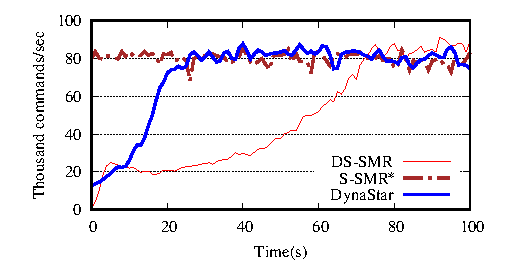
\includegraphics[width=0.95\columnwidth]{figures/experiments/dynastar/socc-tp-strong-locality}
%     \caption{Throughput with strong locality}
%   \end{subfigure}
%   \begin{subfigure}[b]{0.45\textwidth}
%     \centering
%     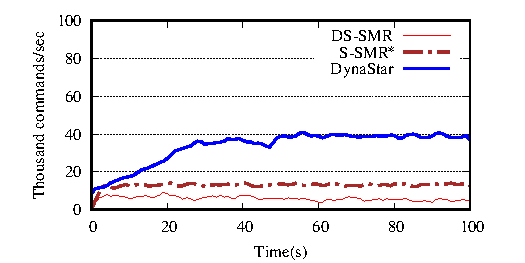
\includegraphics[width=0.95\columnwidth]{figures/experiments/dynastar/socc-tp-weak-locality}
%     \caption{Throughput with weak locality}
%   \end{subfigure} \\
%   \begin{subfigure}[b]{0.45\textwidth}
%     \centering
%     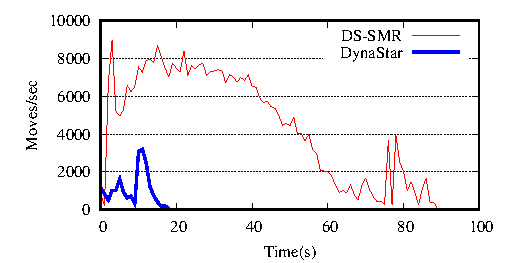
\includegraphics[width=0.95\columnwidth]{figures/experiments/dynastar/socc-moves-strong-locality}
%   \caption{Number of move commands with strong locality}
%   \end{subfigure}
%   \begin{subfigure}[b]{0.45\textwidth}
%     \centering
%     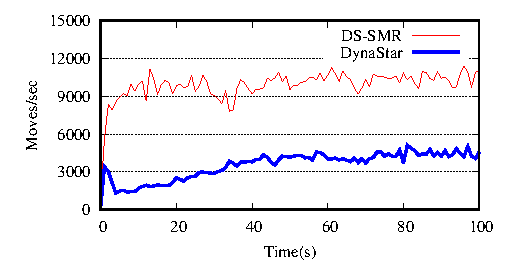
\includegraphics[width=0.95\columnwidth]{figures/experiments/dynastar/socc-moves-weak-locality}
%     \caption{Number of move commands with weak locality}
%   \end{subfigure}
%   \caption{\dynastar, S-SMR* (i.e., optimized S-SMR) and DS-SMR under strong and weak locality, 4 partitions.}
%   \label{fig:motivation}
% \end{figure*}

% \subsection{Static state partitioning with S-SMR}

% \subsection{Dynamic state partitioning}

% Dynamic techniques address the limitations of static techniques by adapting the
% partitioning scheme as workloads change

% There are two general approaches to handle multi-partition commands in terms of
% consistency guarantees. One approach, known as \emph{weak consistency}, is to
% weaken the guarantees of commands that involve multiple partitions (e.g.,
% \cite{facebookTAO}). In the context of SMR, this would mean that requests access
% data within single partition (single-partition commands) are strongly consistent
% (i.e., linearizable), while concurrent requests accessing multiple partitions
% (multi-partition commands) may lead to inconsistencies. This approach relaxes
% the consistency guarantees and makes systems less exposed to impossibility
% results \cite{FLP85, diskpaxos}, but makes the effects of data partitioning and
% replication visible to the application. To lower the chance of potential
% conflicts, data access patterns can be considered when partitioning data (i.e.,
% objects often accessed together can be co-located in the same partition). But
% these optimizations require prior knowledge about the workload, and are often
% performed offline \cite{facebookTAO}

% The other approach, known as \emph{strong consistency}, is to provide strong
% consistency guarantees for both single- and multi-partition commands and hide
% the complexity of data partitioning and replication from the application. The
% algorithms used to implement strong consistency comes with the cost of a more
% complex execution path for commands that involve multiple partitions. Some
% proposals in this category totally order requests before their execution, as in
% state machine replication, or execute requests first and then totally order the
% validation of their execution, as in distributed database systems with
% two-phase-commit.

% \subsection{Partitioning application state}

% Modern distributed systems typically scale performance by partitioning
% application state and tolerate failures by replicating each partition. Clients
% submit commands for execution to one or more partitions. Within a partition,
% replicas coordinate by means of a consensus protocol (e.g., Paxos~\cite{Lam98}).
% To coordinate the execution of multi-partition commands, replicated partitions
% rely on some distributed coordination protocol (e.g., two-phase locking
% \cite{corbett2013spanner}, optimistic concurrency control \cite{Chang:2008},
% atomic multicast \cite{bezerra2014ssmr}).

% In principle, increasing the number of partitions should result in increased
% system performance. However, if the execution of commands involves multiple
% partitions, then performance can actually decrease, due to overhead from
% ordering and coordinating commands across partitions to ensure strong
% consistency. Different techniques have been proposed to handle commands that
% access state in multiple partitions, but inherently multi-partition commands are
% more expensive than single-partition commands. Moreover, if data is not
% distributed carefully, then load imbalances can nullify the benefits of
% partitioning. Thus, an ideal partitioning scheme is one that would both (i)
% allow commands to be executed at a single partition only, and (ii) evenly
% distribute data so that load is balanced among partitions. We refer to workloads
% that can be partitioned in a way that satisfies these two properties as
% exhibiting \emph{strong locality}. Conversely, workloads that cannot avoid
% multi-partition commands with balanced load among partitions exhibit \emph{weak
% locality}.



% \subsection{Static state partitioning with S-SMR}


% \subsection{Dynamic state partitioning}

%\ssmr\ performs better as the number of multi-partition commands decreases.




% Static techniques choose an immutable assignment of application state variables
% to partitions prior to executing commands. Dynamic techniques address the
% limitations of static techniques by adapting the partitioning scheme as
% workloads change. For example, a dynamic technique can move data ``on demand''
% to maximize the number of single partition user commands, while avoiding
% imbalances in the load of the partitions.
% %Typically, this is implemented by moving data ``on demand'' to a single
% %partition which executes a user command.
% The major challenge in designing a dynamic scheme is determining how the system
% selects the partition to which to move data.


% Figure~\ref{fig:motivation} shows the result of a motivating experiment that
% compares two representative systems, one of each class. In the experiment, we
% measured the throughput and number of state moves over time with two different
% workloads: one with strong locality and one with weak locality. The workloads
% are inspired by the social network Twitter, in which the network is modeled as a
% graph, and users can ``post'' messages. The social graph was generated using a
% Zipfian distribution, where the Zipf parameter was adjusted to alter the
% locality.  For brevity, we postpone the details of the experimental setup until
% Section~\ref{sec:experiments}.


% Static techniques choose an immutable assignment of application state variables
% to partitions prior to executing commands. As an example of a static approach
% for use in the experiment, we modified the S-SMR system~\cite{bezerra2014ssmr}
% to use the static METIS~\cite{Abou-Rjeili:2006} partitioning algorithm.  The
% METIS algorithm is optimized to minimize edge-cuts when partitioning a static
% social graph. In the workload with strong locality, METIS partitions the social
% graph such that all posts are single partition; in the workload with weak
% locality, although most commands are single partition, a small fraction of posts
% involves multiple partitions. The throughput is less for the weak locality
% workload due to the more expensive execution of multi-partition posts.
% %since the static scheme incurs overhead when accessing multiple partitions to
% %execute commands.
% For workloads that do not change the graph structure and exhibit strong
% locality, the results for optimized S-SMR in Figure~\ref{fig:motivation} show a
% theoretical maximum throughput.  Of course, these results are not achievable in
% practice, since for real workloads, the graph would change over time (e.g., in
% social networks users join and leave the system, connections are created and
% removed).


% Dynamic techniques address the limitations of static techniques by adapting the
% partitioning scheme as workloads change. For example, a dynamic technique can
% move data ``on demand'' to maximize the number of single partition user
% commands, while avoiding imbalances in the load of the partitions.
% %Typically, this is implemented by moving data ``on demand'' to a single
% %partition which executes a user command.
% The major challenge in designing a dynamic scheme is determining how the system
% selects the partition to which to move data.
% %
% The second system in Figure~\ref{fig:motivation} evaluates DS-SMR, a dynamic
% partitioning strategy implemented by  Le et al.~\cite{le2016dssmr}. This system
% selects partitions randomly, which allows for a completely decentralized
% implementation, in which partitions make only local choices about data movement.
% We refer to this approach as \emph{decentralized dynamic}.  As
% Figure~\ref{fig:motivation} shows, the decentralized dynamic approach works well
% for data with strong locality, but is unstable for workloads with weak locality,
% since data is constantly moved from one partition to another.
